For the plots presented in this results section, we will begin displaying data starting from epoch 50.
This way we can evaluate the convergence in the later epochs without the low accuracy/$R^2$ in the first few epochs completely dominating the plots.

\subsection{Franke function data}

\subsubsection{Neural network}

Based on the initial search, using the momentum optimizer seems to be a good choice for further investigation.
Furthermore, we note that the Adam optimizer and the RMSprop optimizer make up the best three together with the momentum optimizer.

\begin{figure}[h!]
    \centering
    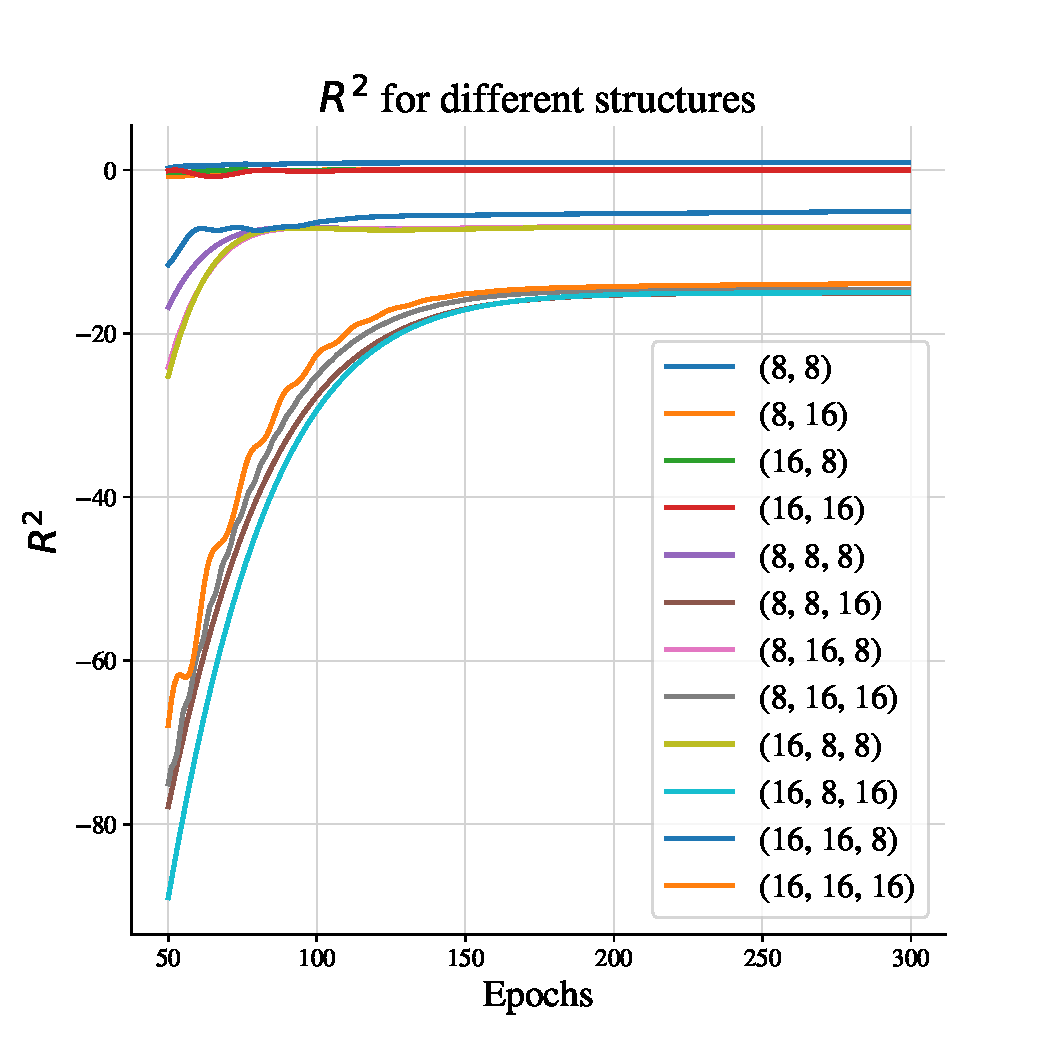
\includegraphics[width=1.0\linewidth]{project_2/figures/$R^2$ for different structures_continuous.pdf}
    \caption{$R^2$ for the neural network for different number of layers and sizes for each layer. The best one is (24,24).}
    \label{fig:structure_franke}
\end{figure}

Fig. \ref{fig:structure_franke} shows the $R^2$ for models with different network structures, but otherwise the same parameters. It is interesting to notice that for two layers with a size of 24 each we get the model which yields the highest $R^2$ score. We tested for two and three layers and layer sizes of 8 and 24. 
It seems fewer, but bigger layers are favorable. 
The reason for this might be that due to the large amount of noise, deeper networks might be prone to overfitting.
A network with few but wide layers allows for capturing complex interactions, while still being shallow enough to avoid over-complication and overfitting.

\begin{figure}[h!]
    \centering
    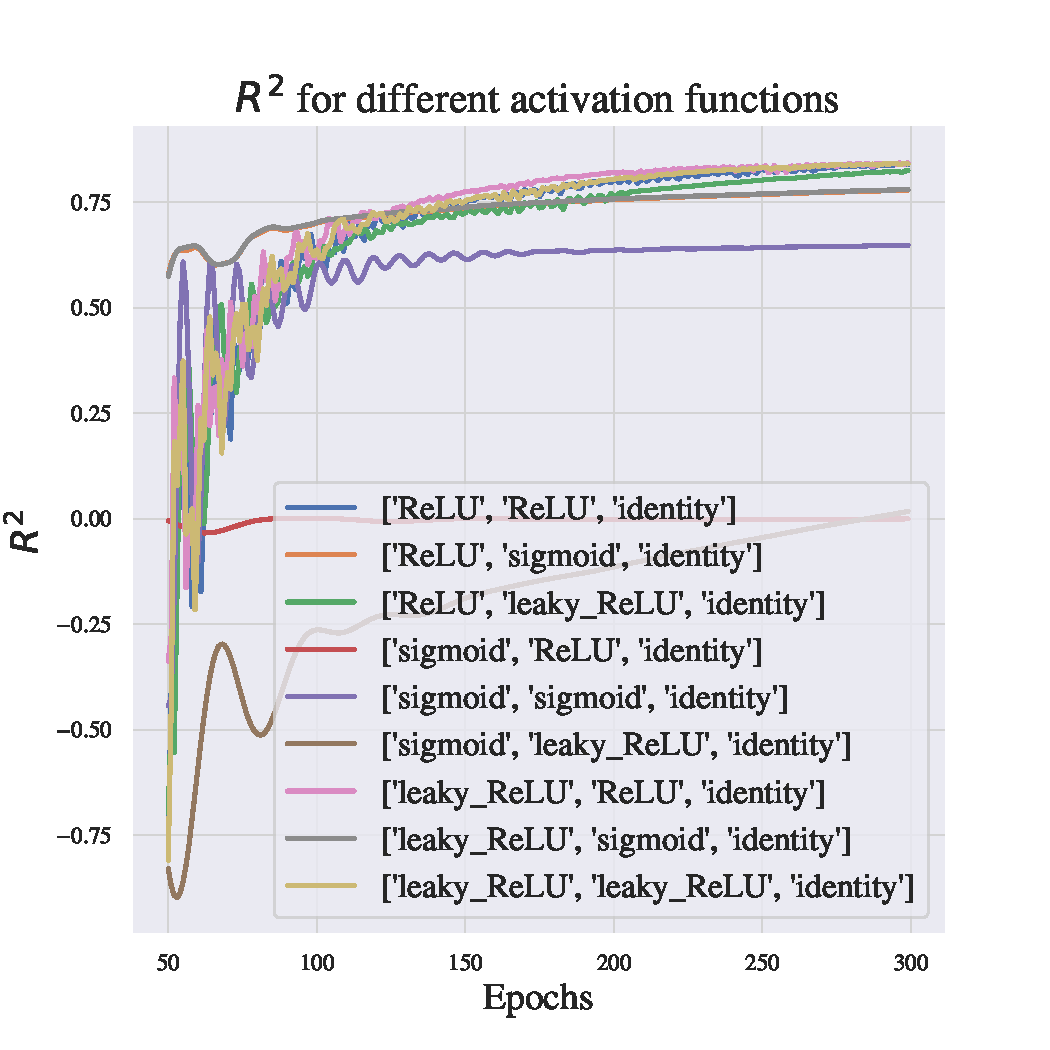
\includegraphics[width=1.0\linewidth]{project_2/figures/$R^2$ for different activation functions_continuous.pdf}
    \caption{The $R^2$ for different choices of activation functions for the two hidden layers. Identity is always used as the final activation function. The best $R^2$ is found when we use leaky ReLU at the first hidden layer and ReLU at the second.}
    \label{fig:activation_franke}
\end{figure}

Using the network structure found in the previous step, we try different activation functions for the two hidden layers. 
Fig. \ref{fig:activation_franke} visualizes how the different models perform. 
The three worst performing models are those with sigmoid as the activation function at the first hidden layer. 
This is likely due to the fact that sigmoid is not designed for problems where one might want target values outside the range [0,1].
In the case where the sigmoid outputs something close to 1, and the backpropagation pushes it to become even larger, we might experience vanishing gradients, causing the training to halt before our wanted convergence point.
The four best ones are the ones that combines leaky ReLU and ReLU (both orders) and just one or the other. 
The very best model has leaky ReLU at the first hidden layer and ReLU and the second.

\begin{figure}[h!]
    \centering
    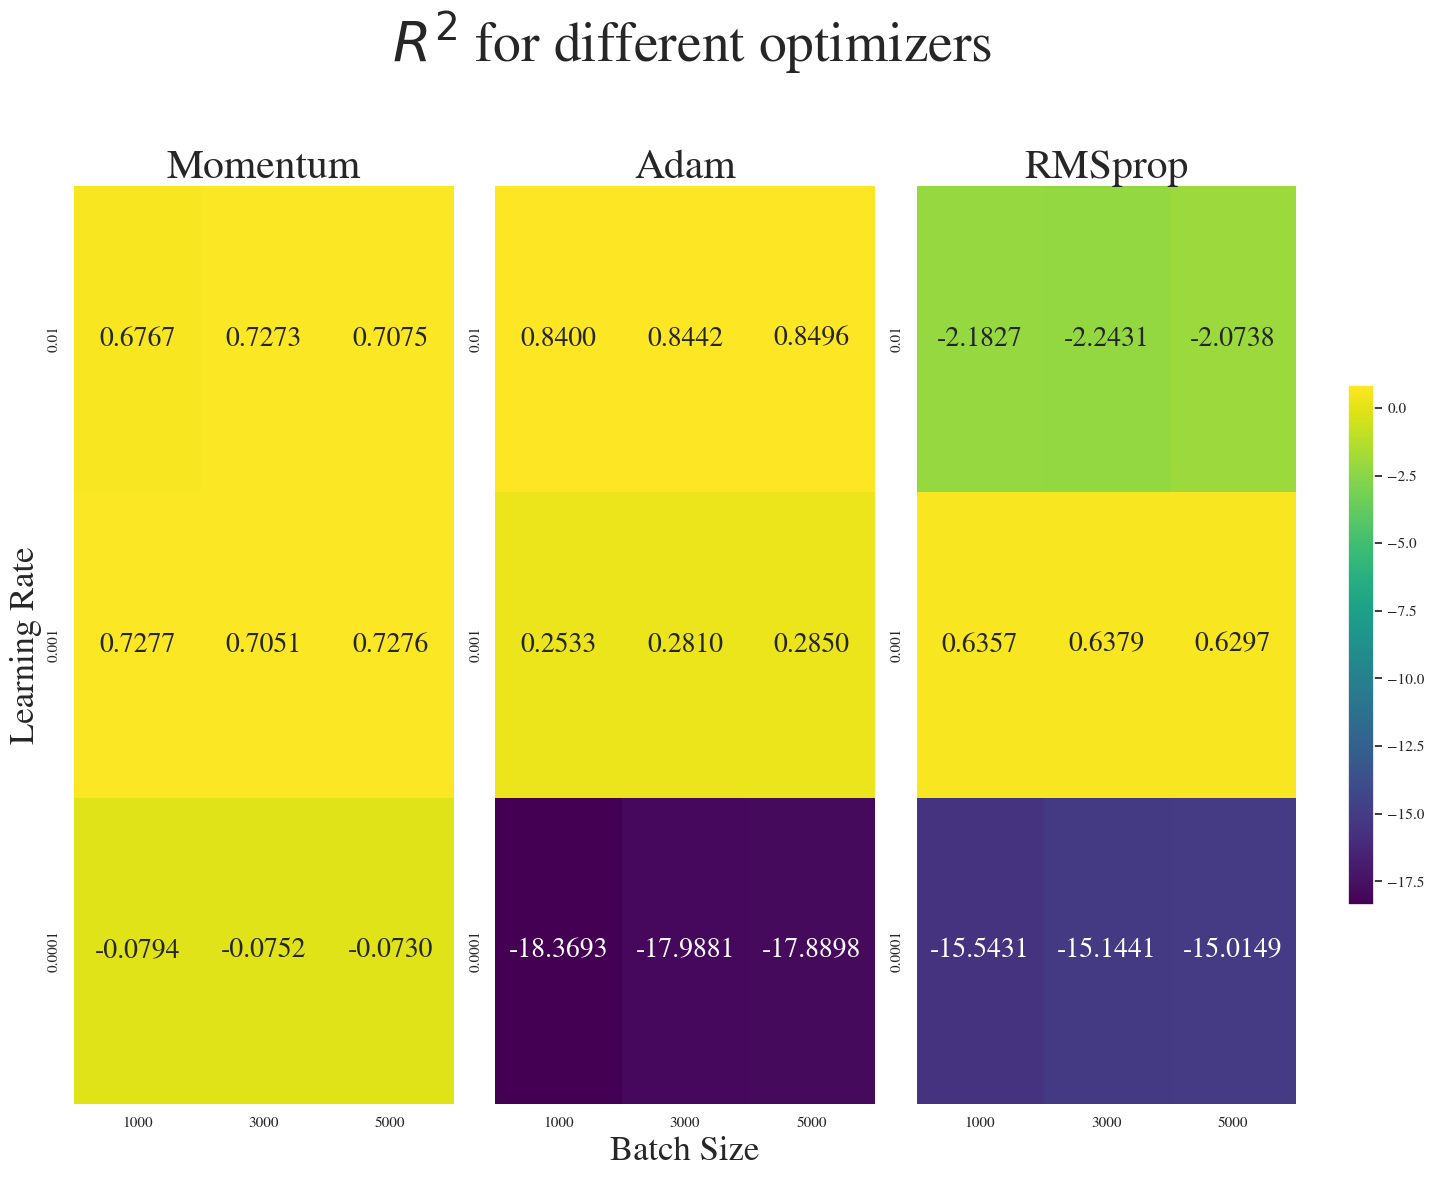
\includegraphics[width=1.0\linewidth]{project_2/figures/r2_grid_final.png}
    \caption{The $R^2$ on the test set for different sets of learning rates and batch sizes for the three best optimizers.}
    \label{fig:grid_franke}
\end{figure}

Using (2,24,24,1) as the network structure and (leaky ReLU, ReLU, identity) as the activation functions, the grid search for the best combination of initial learning rate and batch size is shown in Fig. \ref{fig:grid_franke}. The three best optimizers, momentum, Adam, and RMSprop, are used. 
We look for the combination that gives the highest $R^2$ on the test set for each of the optimizers. 

For both momentum and RMSProp, the optimal seems to be a balanced learning rate of order of magnitude $10^{-3}$.
For the Adam optimizer however, a higher learning rate of magnitude $10^{-2}$ is preferred.
%As momentum has an extra term adding to the gradient, while RMSProp divides the gradient on a factor larger than one, we would have expected the optimal learning rates of these models to be on either side of that of the constant optimizer (momentum being lower, RMSProp higher).

The best combination of learning rate and batch size for the Adam optimizer is (0.01, 5000). For the momentum optimizer we find it to be (0.001, 5000). Lastly, the model trained with RMSprop optimizer obtains the highest $R^2$ with the combination (0.001,5000). 
The impact of the batch size is not very large, but a batch size of 5000 slightly outperforms both 1000 and 3000 in all nine cases represented in Fig. \ref{fig:grid_franke}. 
As the $R^2$ is similar across batch sizes, it may seem that 1000 data points is enough to get a representative subset of the total data, but that 5000 provides a small advantage. 
%which could be due to the case that 1000 data points is enough to get a representative subset of the total data.
%Smaller batch sizes performing slightly better could be due to some degree of randomness improving the learning steps.


\begin{figure}[h!]
    \centering
    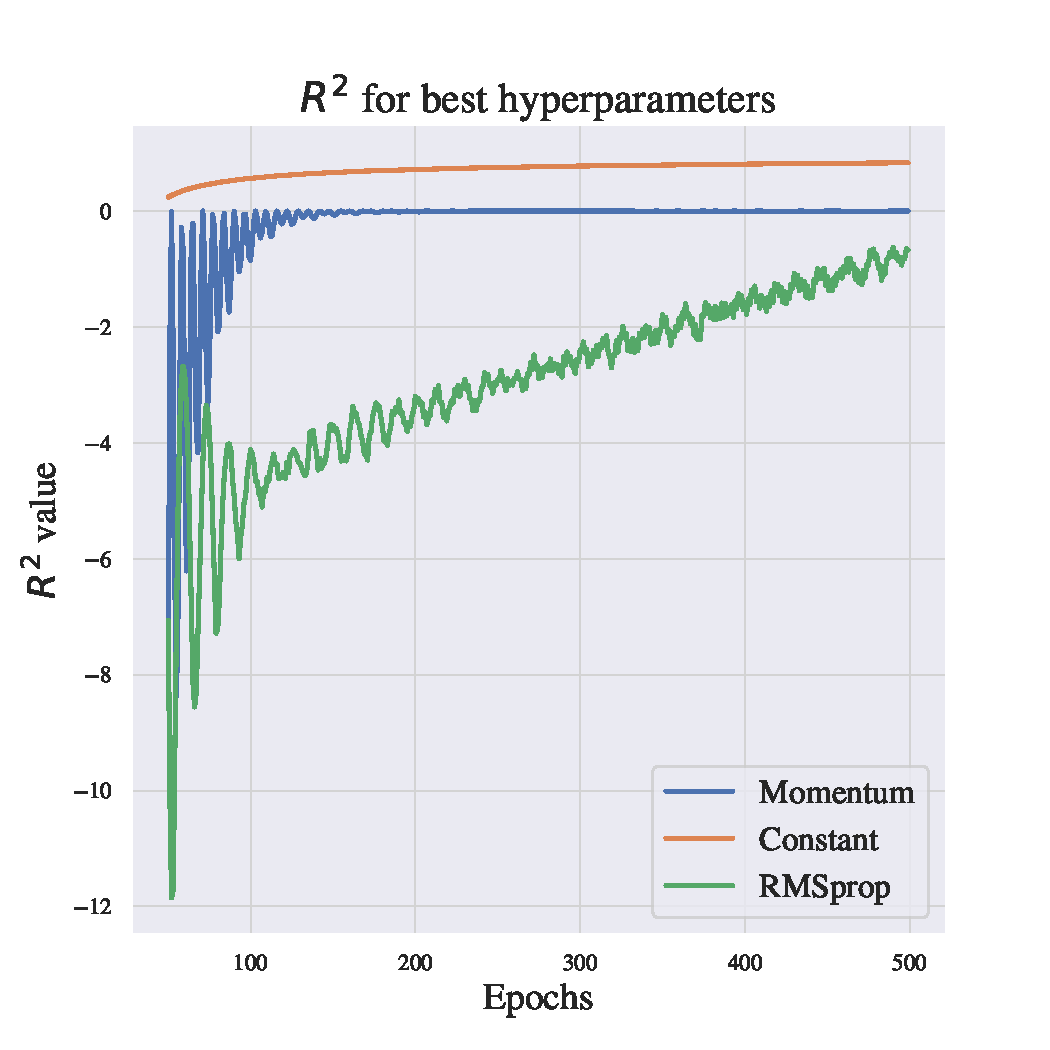
\includegraphics[width=1.0\linewidth]{project_2/figures/best_continuous.pdf}
    \caption{The $R^2$ on the test set for the final three models.}
    \label{fig:best_franke}
\end{figure}

The best model reaches an $R^2$ score of $0.85$. This model is trained with the Adam optimizer as seen in Fig. \ref{fig:best_franke}.

\subsubsection{Comparison to linear regression}


In our previous work, \textcite{project1}, the maximal $R^2$ for the ordinary least squares model was found to be $0.86$. 
This is a slightly higher value than obtained from the neural network. 

By calculating the $R^2$ between the Franke function data with no noise and the one with noise, we find a value of 0.89. 
This can be considered the maximum attainable $R^2$ for a dataset with this level of noise, disregarding any lucky results that might push the value higher, i.e. how much of the noise in the data is theoretically explainable.

Values of $0.85$ and $0.86$ for the neural network and the linear regression model respectively, are therefore very good. 

%This is far lower than the $R^2 = 0.83$ obtained from the neural network.
%This shows that our neural network model performs substantially better than any linear regression model.
%The added flexibility and possible complexity in the neural networks make them superior to linear regression when the data to be modeled does not contain linear dependencies.

\subsection{Breast cancer data}

\subsubsection{Neural network}

Based on the initial search, using the Adam optimizer seems to be a good choice for the further investigation. The optimizers RMSprop and Adagrad with momentum make up the best three together with Adam. 

\begin{figure}[h!]
    \centering
    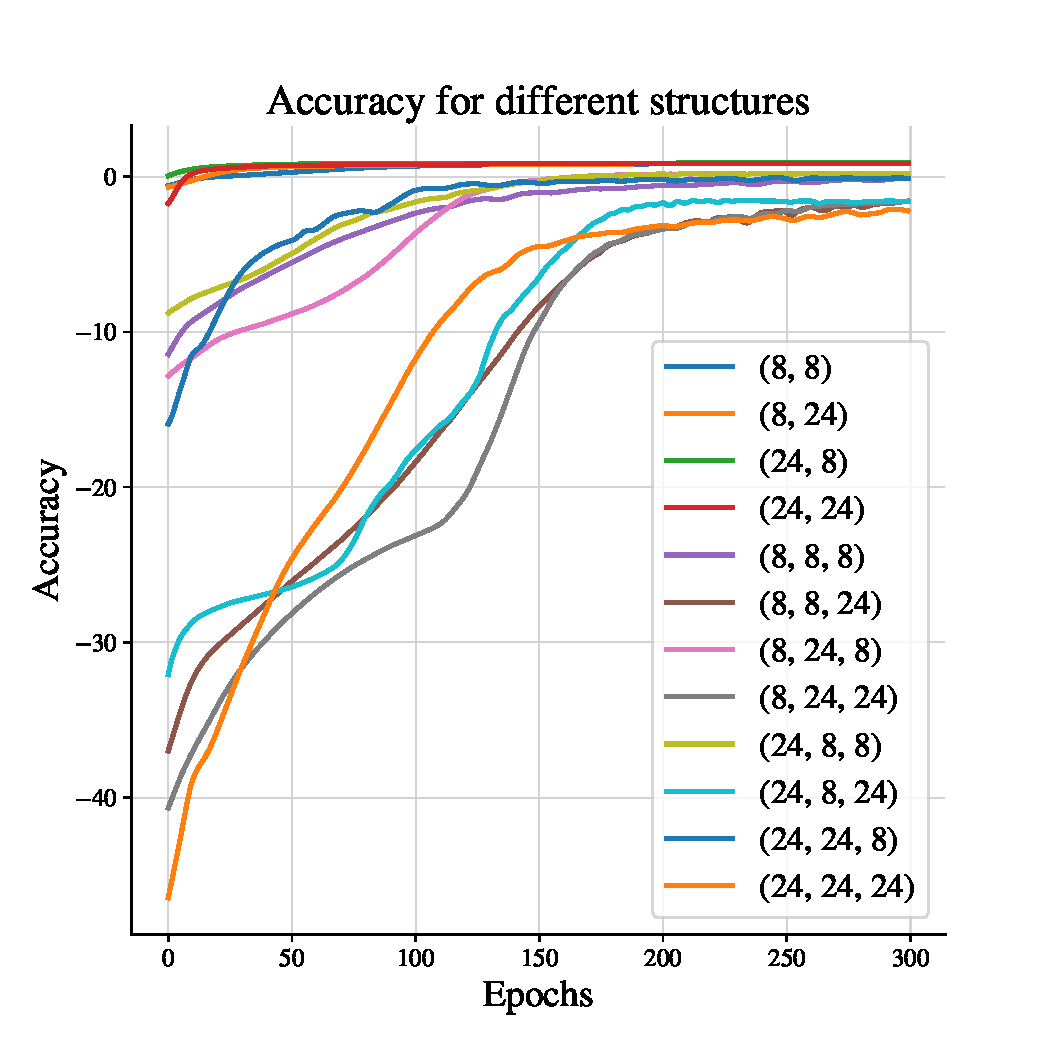
\includegraphics[width=1.0\linewidth]{project_2/figures/Accuracy for different structures_classification.pdf}
    \caption{The accuracy for the neural network for different number of layers and sizes for each layer. The best one is (24,8).}
    \label{fig:structure_cancer}
\end{figure}

Using the Adam optimizer, we test for the best structure of the network. As with the regression problem, two hidden layers are preferred over three. 
The best performing network, the one which gives the highest accuracy, is the one with (24, 8) as the hidden layers. The four best ones are the ones with only two layers, clearly shown on Fig. \ref{fig:structure_cancer}. They majorly outperform the models with three hidden layers. 
The reason for this could again be overfitting in the overly complex models.

\begin{figure}[h!]
    \centering
    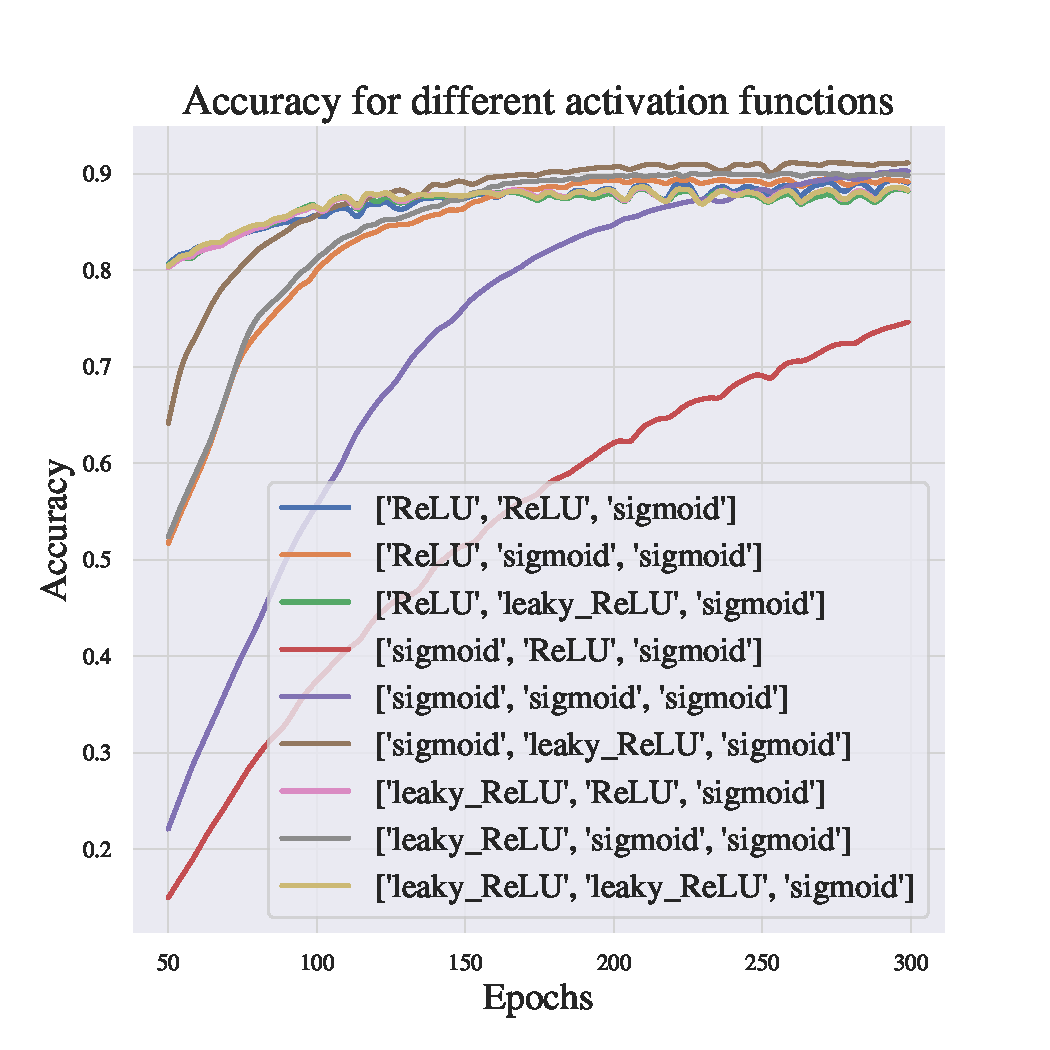
\includegraphics[width=1.0\linewidth]{project_2/figures/Accuracy for different activation functions_classification.pdf}
    \caption{The accuracy for different choices of activation functions for the two hidden layers. Sigmoid is always used as the final activation function. The best $R^2$ is found for (sigmoid, Leaky ReLU).}
    \label{fig:activations_cancer}
\end{figure}

Keeping the two hidden layers of size (24,8), Fig. \ref{fig:activations_cancer} shows how different choices of activation functions for the hidden layers lead to different accuracies. 
Sigmoid is always used as the activation function as the final layer. 
The best model is the one with (sigmoid, leaky ReLU) at the hidden layers. 

\begin{figure}[h!]
    \centering
    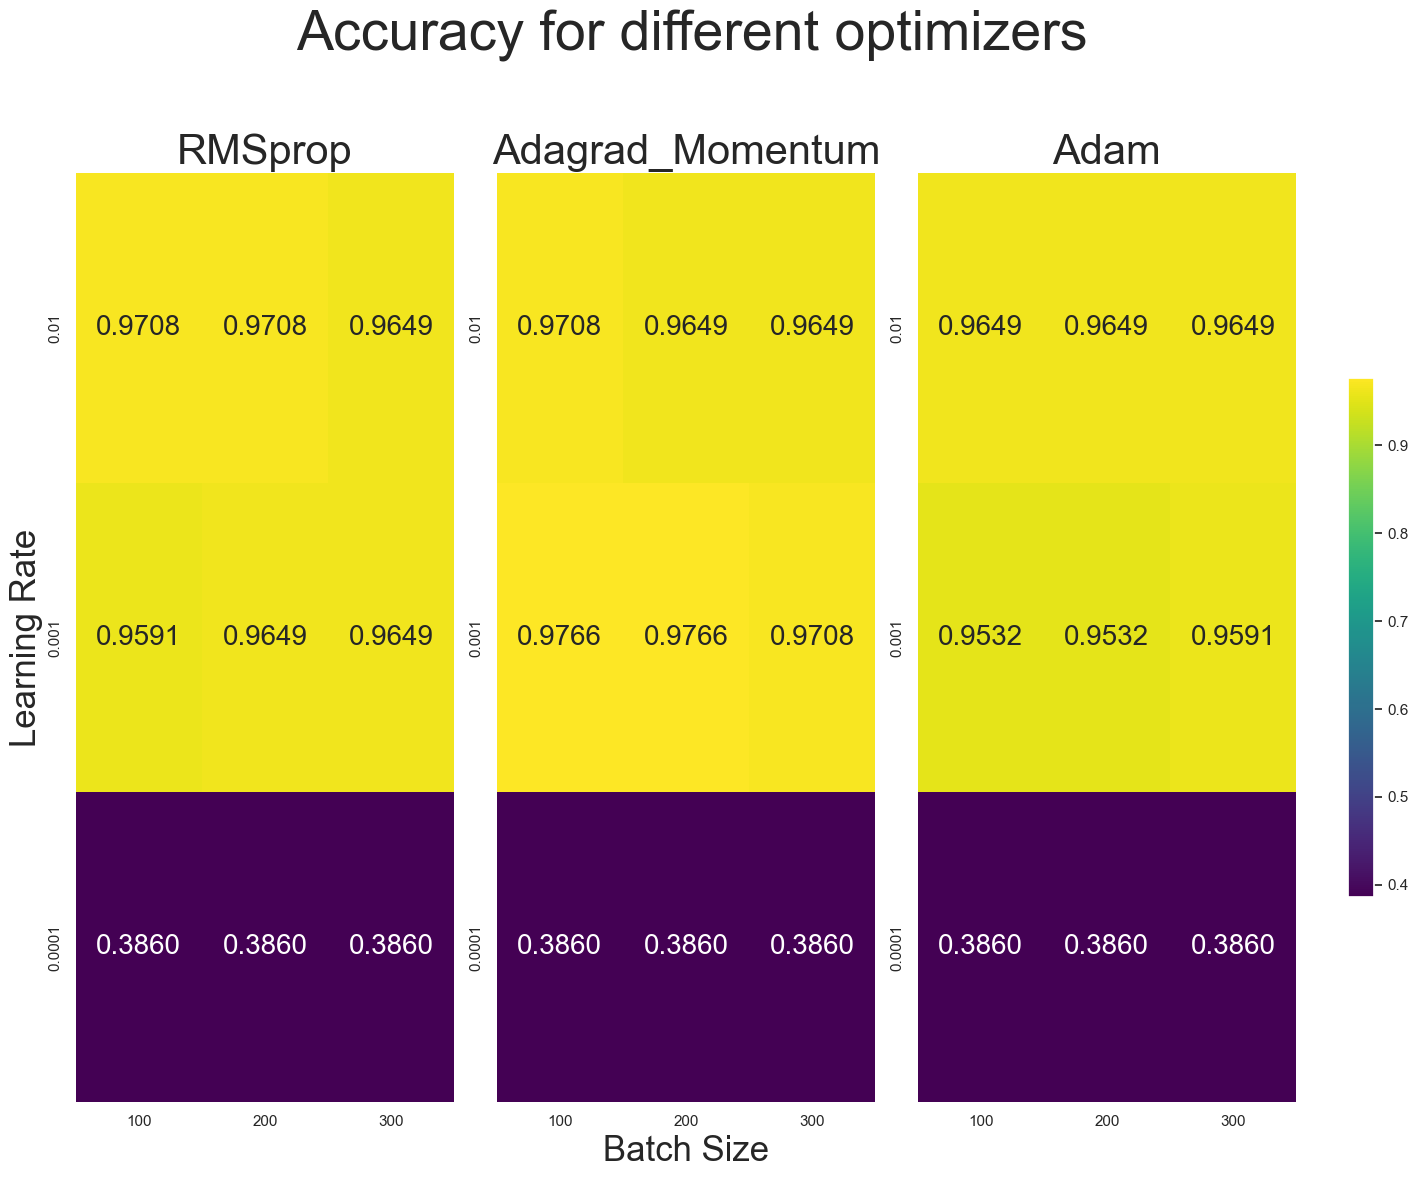
\includegraphics[width=1.0\linewidth]{project_2/figures/acc_grid_clas.png}
    \caption{The accuracy on the test set for different sets of learning rates and batch sizes for the three best optimizers.}    
    \label{fig:grid_cancer}
\end{figure}

Given a network structure of (30,24,8,1) and (sigmoid, leaky ReLU, sigmoid) as the activation functions, we tested for the best combination of learning rate and batch size for each of the three best optimizers.
We get the best results using AdaGrad with momentum, with learning rate 0.001, and batch sizes 100 and 200 performing exactly equal.
Note that as we only test this on a test set containing 171 data points, the accuracy will follow a seemingly very discrete scheme according to number of correct predictions divided by 171, hence it is expected to see different models with the exact same accuracy.
It is possible that the models with learning rate 0.0001 are all caught by the same local minima.

\begin{figure}[h!]
    \centering
    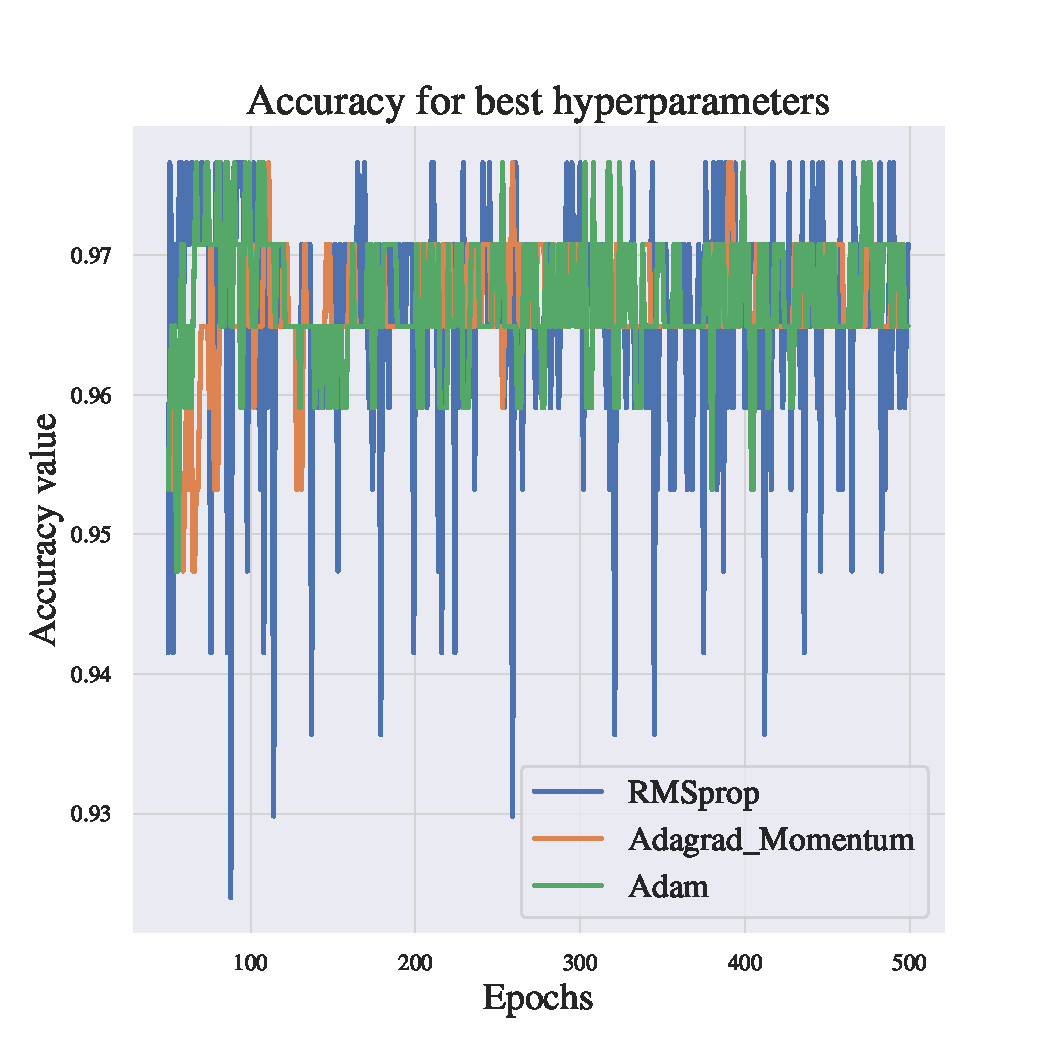
\includegraphics[width=1.0\linewidth]{project_2/figures/best_classification.pdf}
    \caption{The accuracy on the test set for the final three models.}
    \label{fig:best_cancer}
\end{figure}

The best model for the classification problem given our method of exploring the different aspects, gives an accuracy of $0.97$.
This is the with RMSprop optimizer. 

In Fig. \ref{fig:best_cancer} we clearly see the issue with having a small data set: each of the seemingly large jumps in accuracy does indeed represent just one patient each.
It is not unexpected to see the models losing/gaining one correct prediction while closing in on its point of convergence, it simply looks weird in this case due to few data points.

\subsubsection{Comparison to logistic regression}

Our final logistic regression model has an accuracy of $0.97$. This is the same as for the neural network. 

We will consider the additional metrics recall, precision and F-score. These are presented in table \ref{tab:class_score}.

\begin{table}[h]
    \centering
    \begin{tabular}{|m{8em}|m{8.5em}|m{8.5em}|}
    \hline
         & \textbf{NN} & \textbf{LogReg} \\
    \hline
        \textbf{Accuracy} & 0.97 & 0.97\\
    \hline
        \textbf{Precision} & 0.98 & 0.96 \\
    \hline
        \textbf{Recall} & 0.94 & 0.97 \\
    \hline
        \textbf{F-score} & 0.96 & 0.96 \\
    \hline
    \end{tabular}
    \caption{Scores for classification problem}
    \label{tab:class_score}
\end{table}

We see that both models has the exact same accuracy; predicting 166 of the 171 test subjects correctly.
They also achieve identical F-scores, hence one could say that they are equally good.
However, when looking at the precision, we observe that the neural network is performing slightly better.
For the recall, the logistic regression slightly outperforms the neural network.
As the discussion in section \ref{sec:meas_class} concluded, all errors are not equally bad; in particular it is worse to predict an ill patient to be healthy than the opposite.

In this case, the recall is thus more important than the precision, since the recall tells how many of the ill patients are predicted to be ill.
The difference between the two models is that while both are as likely to perform a correct prediction for a randomly chosen patient, the neural network is slightly more likely to categorize an ill person as healthy, while the logistic regression model categorizes more healthy patients as ill.
As discussed, it is quite clear that you would rather want the latter.
This, combined with the logistic regression model being easier to design, requiring less tuning and being easier to interpret, we find this to be the better model.

Since a logistic regression model technically is a neural network with no hidden layers, we clearly could have found a better neural network than we did.
We do believe that a way to possibly design better neural networks for this task, is to replace our current loss function by one punishing false negatives harder than false positive, making the model prone to prioritize a high recall over high precision.